\documentclass[letterpaper, 12pt]{article}

% --- Package imports ---

% Extended set of colors
\usepackage[dvipsnames]{xcolor}
\usepackage{tikz}
\usepackage{graphicx}
\usepackage{float}
\usepackage{
  amsmath, amsthm, amssymb, mathtools, dsfont, units,          % Math typesetting
  graphicx, wrapfig, subfig, float,                            % Figures and graphics formatting
  listings, color, inconsolata, pythonhighlight,               % Code formatting
  fancyhdr, sectsty, hyperref, enumerate, enumitem, framed }   % Headers/footers, section fonts, links, lists

% lipsum is just for generating placeholder text and can be removed
\usepackage{hyperref, lipsum} 

% --- Fonts ---

\usepackage{newpxtext, newpxmath, inconsolata}

% --- Page layout settings ---

% Set page margins
\usepackage[left=1.35in, right=1.35in, top=1.0in, bottom=.9in, headsep=.2in, footskip=0.35in]{geometry}

% Anchor footnotes to the bottom of the page
\usepackage[bottom]{footmisc}

% Set line spacing
\renewcommand{\baselinestretch}{1.2}

% Set spacing between paragraphs
\setlength{\parskip}{1.3mm}

% Allow multi-line equations to break onto the next page
\allowdisplaybreaks

% --- Page formatting settings ---

% Set image captions to be italicized
\usepackage[font={it,footnotesize}]{caption}

% Set link colors for labeled items (blue), citations (red), URLs (orange)
\hypersetup{colorlinks=true, linkcolor=RoyalBlue, citecolor=RedOrange, urlcolor=ForestGreen}

% Set font size for section titles (\large) and subtitles (\normalsize) 
\usepackage{titlesec}
\titleformat{\section}{\large\bfseries}{{\fontsize{19}{19}\selectfont\textreferencemark}\;\; }{0em}{}
\titleformat{\subsection}{\normalsize\bfseries\selectfont}{\thesubsection\;\;\;}{0em}{}

% Enumerated/bulleted lists: make numbers/bullets flush left
%\setlist[enumerate]{wide=2pt, leftmargin=16pt, labelwidth=0pt}
\setlist[itemize]{wide=0pt, leftmargin=16pt, labelwidth=10pt, align=left}

% --- Table of contents settings ---

\usepackage[subfigure]{tocloft}

% Reduce spacing between sections in table of contents
\setlength{\cftbeforesecskip}{.9ex}

% Remove indentation for sections
\cftsetindents{section}{0em}{0em}

% Set font size (\large) for table of contents title
\renewcommand{\cfttoctitlefont}{\large\bfseries}

% Remove numbers/bullets from section titles in table of contents
\makeatletter
\renewcommand{\cftsecpresnum}{\begin{lrbox}{\@tempboxa}}
\renewcommand{\cftsecaftersnum}{\end{lrbox}}
\makeatother

% --- Set path for images ---

\graphicspath{{Images/}{../Images/}}

% --- Math/Statistics commands ---

% Add a reference number to a single line of a multi-line equation
% Usage: "\numberthis\label{labelNameHere}" in an align or gather environment
\newcommand\numberthis{\addtocounter{equation}{1}\tag{\theequation}}

% Shortcut for bold text in math mode, e.g. $\b{X}$
\let\b\mathbf

% Shortcut for bold Greek letters, e.g. $\bg{\beta}$
\let\bg\boldsymbol

% Shortcut for calligraphic script, e.g. %\mc{M}$
\let\mc\mathcal

% \mathscr{(letter here)} is sometimes used to denote vector spaces
\usepackage[mathscr]{euscript}

% Convergence: right arrow with optional text on top
% E.g. $\converge[p]$ for converges in probability
\newcommand{\converge}[1][]{\xrightarrow{#1}}

% Weak convergence: harpoon symbol with optional text on top
% E.g. $\wconverge[n\to\infty]$
\newcommand{\wconverge}[1][]{\stackrel{#1}{\rightharpoonup}}

% Equality: equals sign with optional text on top
% E.g. $X \equals[d] Y$ for equality in distribution
\newcommand{\equals}[1][]{\stackrel{\smash{#1}}{=}}

% Normal distribution: arguments are the mean and variance
% E.g. $\normal{\mu}{\sigma}$
\newcommand{\normal}[2]{\mathcal{N}\left(#1,#2\right)}

% Uniform distribution: arguments are the left and right endpoints
% E.g. $\unif{0}{1}$
\newcommand{\unif}[2]{\text{Uniform}(#1,#2)}

% Independent and identically distributed random variables
% E.g. $ X_1,...,X_n \iid \normal{0}{1}$
\newcommand{\iid}{\stackrel{\smash{\text{iid}}}{\sim}}

% Sequences (this shortcut is mostly to reduce finger strain for small hands)
% E.g. to write $\{A_n\}_{n\geq 1}$, do $\bk{A_n}{n\geq 1}$
\newcommand{\bk}[2]{\{#1\}_{#2}}

% Math mode symbols for common sets and spaces. Example usage: $\R$
\newcommand{\R}{\mathbb{R}}	% Real numbers
\newcommand{\C}{\mathbb{C}}	% Complex numbers
\newcommand{\Q}{\mathbb{Q}}	% Rational numbers
\newcommand{\Z}{\mathbb{Z}}	% Integers
\newcommand{\N}{\mathbb{N}}	% Natural numbers
\newcommand{\F}{\mathcal{F}}	% Calligraphic F for a sigma algebra
\newcommand{\El}{\mathcal{L}}	% Calligraphic L, e.g. for L^p spaces

% Math mode symbols for probability
\newcommand{\pr}{\mathbb{P}}	% Probability measure
\newcommand{\E}{\mathbb{E}}	% Expectation, e.g. $\E(X)$
\newcommand{\var}{\text{Var}}	% Variance, e.g. $\var(X)$
\newcommand{\cov}{\text{Cov}}	% Covariance, e.g. $\cov(X,Y)$
\newcommand{\corr}{\text{Corr}}	% Correlation, e.g. $\corr(X,Y)$
\newcommand{\B}{\mathcal{B}}	% Borel sigma-algebra

% Other miscellaneous symbols
\newcommand{\tth}{\text{th}}	% Non-italicized 'th', e.g. $n^\tth$
\newcommand{\Oh}{\mathcal{O}}	% Big-O notation, e.g. $\O(n)$
\newcommand{\1}{\mathds{1}}	% Indicator function, e.g. $\1_A$

% Additional commands for math mode
\DeclareMathOperator*{\argmax}{argmax}		% Argmax, e.g. $\argmax_{x\in[0,1]} f(x)$
\DeclareMathOperator*{\argmin}{argmin}		% Argmin, e.g. $\argmin_{x\in[0,1]} f(x)$
\DeclareMathOperator*{\spann}{Span}		% Span, e.g. $\spann\{X_1,...,X_n\}$
\DeclareMathOperator*{\bias}{Bias}		% Bias, e.g. $\bias(\hat\theta)$
\DeclareMathOperator*{\ran}{ran}			% Range of an operator, e.g. $\ran(T) 
\DeclareMathOperator*{\dv}{d\!}			% Non-italicized 'with respect to', e.g. $\int f(x) \dv x$
\DeclareMathOperator*{\diag}{diag}		% Diagonal of a matrix, e.g. $\diag(M)$
\DeclareMathOperator*{\trace}{trace}		% Trace of a matrix, e.g. $\trace(M)$
\DeclareMathOperator*{\supp}{supp}		% Support of a function, e.g., $\supp(f)$

% Numbered theorem, lemma, etc. settings - e.g., a definition, lemma, and theorem appearing in that 
% order in Lecture 2 will be numbered Definition 2.1, Lemma 2.2, Theorem 2.3. 
% Example usage: \begin{theorem}[Name of theorem] Theorem statement \end{theorem}
\theoremstyle{definition}
\newtheorem{theorem}{Theorem}[section]
\newtheorem{proposition}[theorem]{Proposition}
\newtheorem{lemma}[theorem]{Lemma}
\newtheorem{corollary}[theorem]{Corollary}
\newtheorem{definition}[theorem]{Definition}
\newtheorem{example}[theorem]{Example}
\newtheorem{remark}[theorem]{Remark}

% Un-numbered theorem, lemma, etc. settings
% Example usage: \begin{lemma*}[Name of lemma] Lemma statement \end{lemma*}
\newtheorem*{theorem*}{Theorem}
\newtheorem*{proposition*}{Proposition}
\newtheorem*{lemma*}{Lemma}
\newtheorem*{corollary*}{Corollary}
\newtheorem*{definition*}{Definition}
\newtheorem*{example*}{Example}
\newtheorem*{remark*}{Remark}
\newtheorem*{claim}{Claim}

% --- Left/right header text (to appear on every page) ---

% Do not include a line under header or above footer
\pagestyle{fancy}
\renewcommand{\footrulewidth}{0pt}
\renewcommand{\headrulewidth}{0pt}

% Right header text: Lecture number and title
\renewcommand{\sectionmark}[1]{\markright{#1} }
\fancyhead[R]{\small\textit{\nouppercase{\rightmark}}}

% Left header text: Short course title, hyperlinked to table of contents
\fancyhead[L]{\hyperref[sec:contents]{\small Introduction}}

% --- Document starts here ---

\begin{document}

% --- Main title and subtitle ---

\title{01-Introduction \\[1em]
\normalsize GSF-3100 \\ Marchés des Capitaux}

% --- Author and date of last update ---

\author{\normalsize Simon-Pierre Boucher}
\date{\normalsize\vspace{-1ex} Last updated: \today}

% --- Add title and table of contents ---

\maketitle
\tableofcontents\label{sec:contents}

% --- Main content: import lectures as subfiles ---

\newpage

\section{Le rôle et les objectifs du marchés financier}
\begin{itemize}

\item Une économie productive exige des entreprises qu'elles produisent des biens et des services destinés à la consommation, et ces entreprises ont besoin de ressources. C'est le marché financier qui relie les besoins en ressources de ces entreprises aux personnes disposées à fournir les ressources nécessaires : sous forme d'investissements.

\item Le système financier existe pour faciliter la conception, la vente et l'échange de fonds et d'investissements financiers. Ce système d'échange prend l'une de deux formes : directe et indirecte. Dans le système d'échange direct (financement), les emprunteurs (émetteurs) vendent des titres directement aux prêteurs (acheteurs). Les emprunteurs comprennent les gouvernements centraux, les gouvernements locaux et les entreprises. Les prêteurs, quant à eux, comprennent les particuliers, les institutions financières et non financières et d'autres gouvernements.

\item Dans les systèmes d'échange indirect (financement), les institutions financières telles que les banques facilitent le transfert de fonds entre les emprunteurs et les prêteurs, en empruntant auprès des prêteurs et en fournissant ensuite les fonds aux emprunteurs finaux. Ces institutions financières sont appelées intermédiaires et comprennent les banques, les compagnies d'assurance et les fonds communs de placement.

\item Il faut remarquer que le système financier est fortement lié au système économique. Le rôle du système financier à cet égard est de faciliter la production, l'emploi et la consommation. Ces liens peuvent être représentés graphiquement comme suit :
\end{itemize}
\begin{figure}[H]
  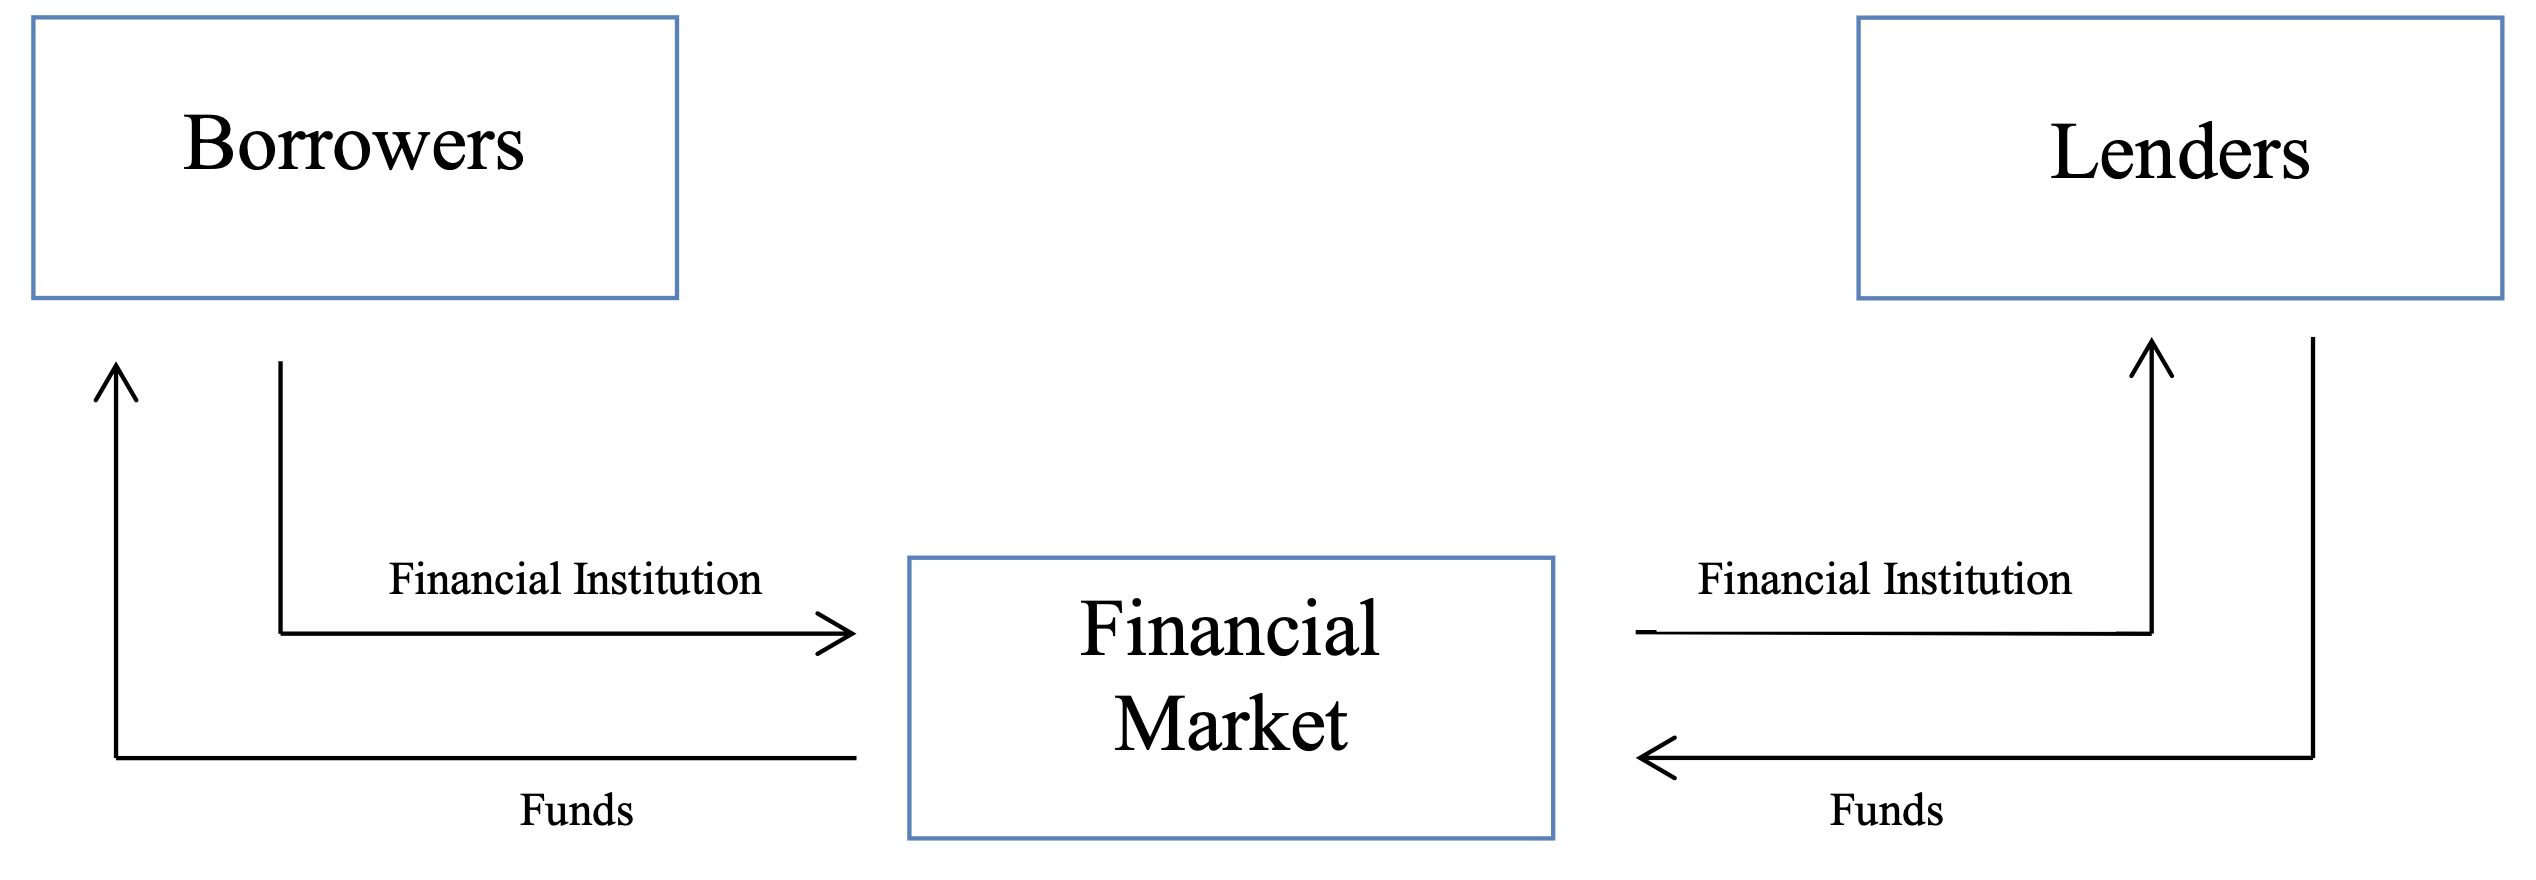
\includegraphics[width=\linewidth]{FIG1a}
  \caption{The Funds Indirect Flow Process}
  \label{fig:boat1}
\end{figure}
\begin{figure}[H]
  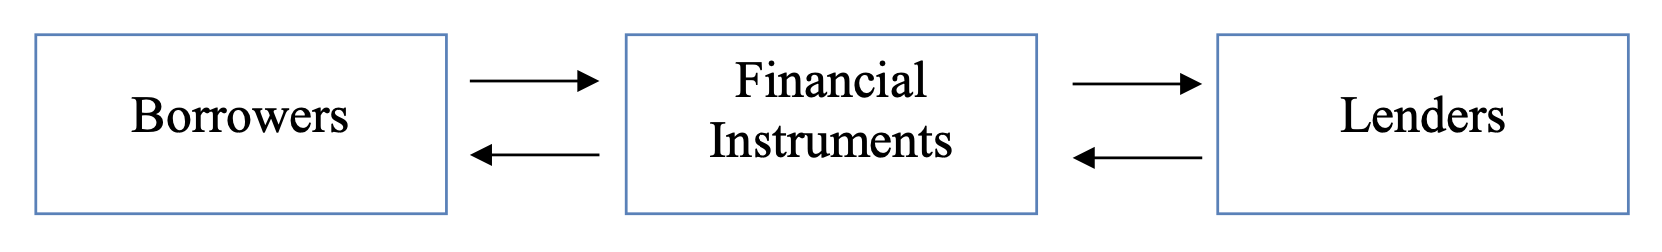
\includegraphics[width=\linewidth]{FIG1b}
  \caption{The Funds Direct Flow Process}
  \label{fig:boat1}
\end{figure}

Au sens large, un investissement est l'engagement actuel d'argent ou d'autres ressources dans l'attente de bénéfices futurs. Un investissement peut être un actif financier ou un actif réel. Les actifs financiers, tels que les actions et les obligations, jouent le rôle essentiel de mise en relation des investisseurs avec les entreprises ayant besoin de ressources pour permettre le bon fonctionnement de l'économie. Les actifs réels, d'autre part, sont les actifs (par exemple, les immobilisations corporelles) qui sont achetés par les entreprises pour produire réellement des biens et des services pour les consommateurs. Outre la mise en relation des entreprises avec les investisseurs, les marchés financiers jouent également un rôle important dans l'évaluation et l'échange d'actifs financiers et réels.

\begin{figure}[H]
  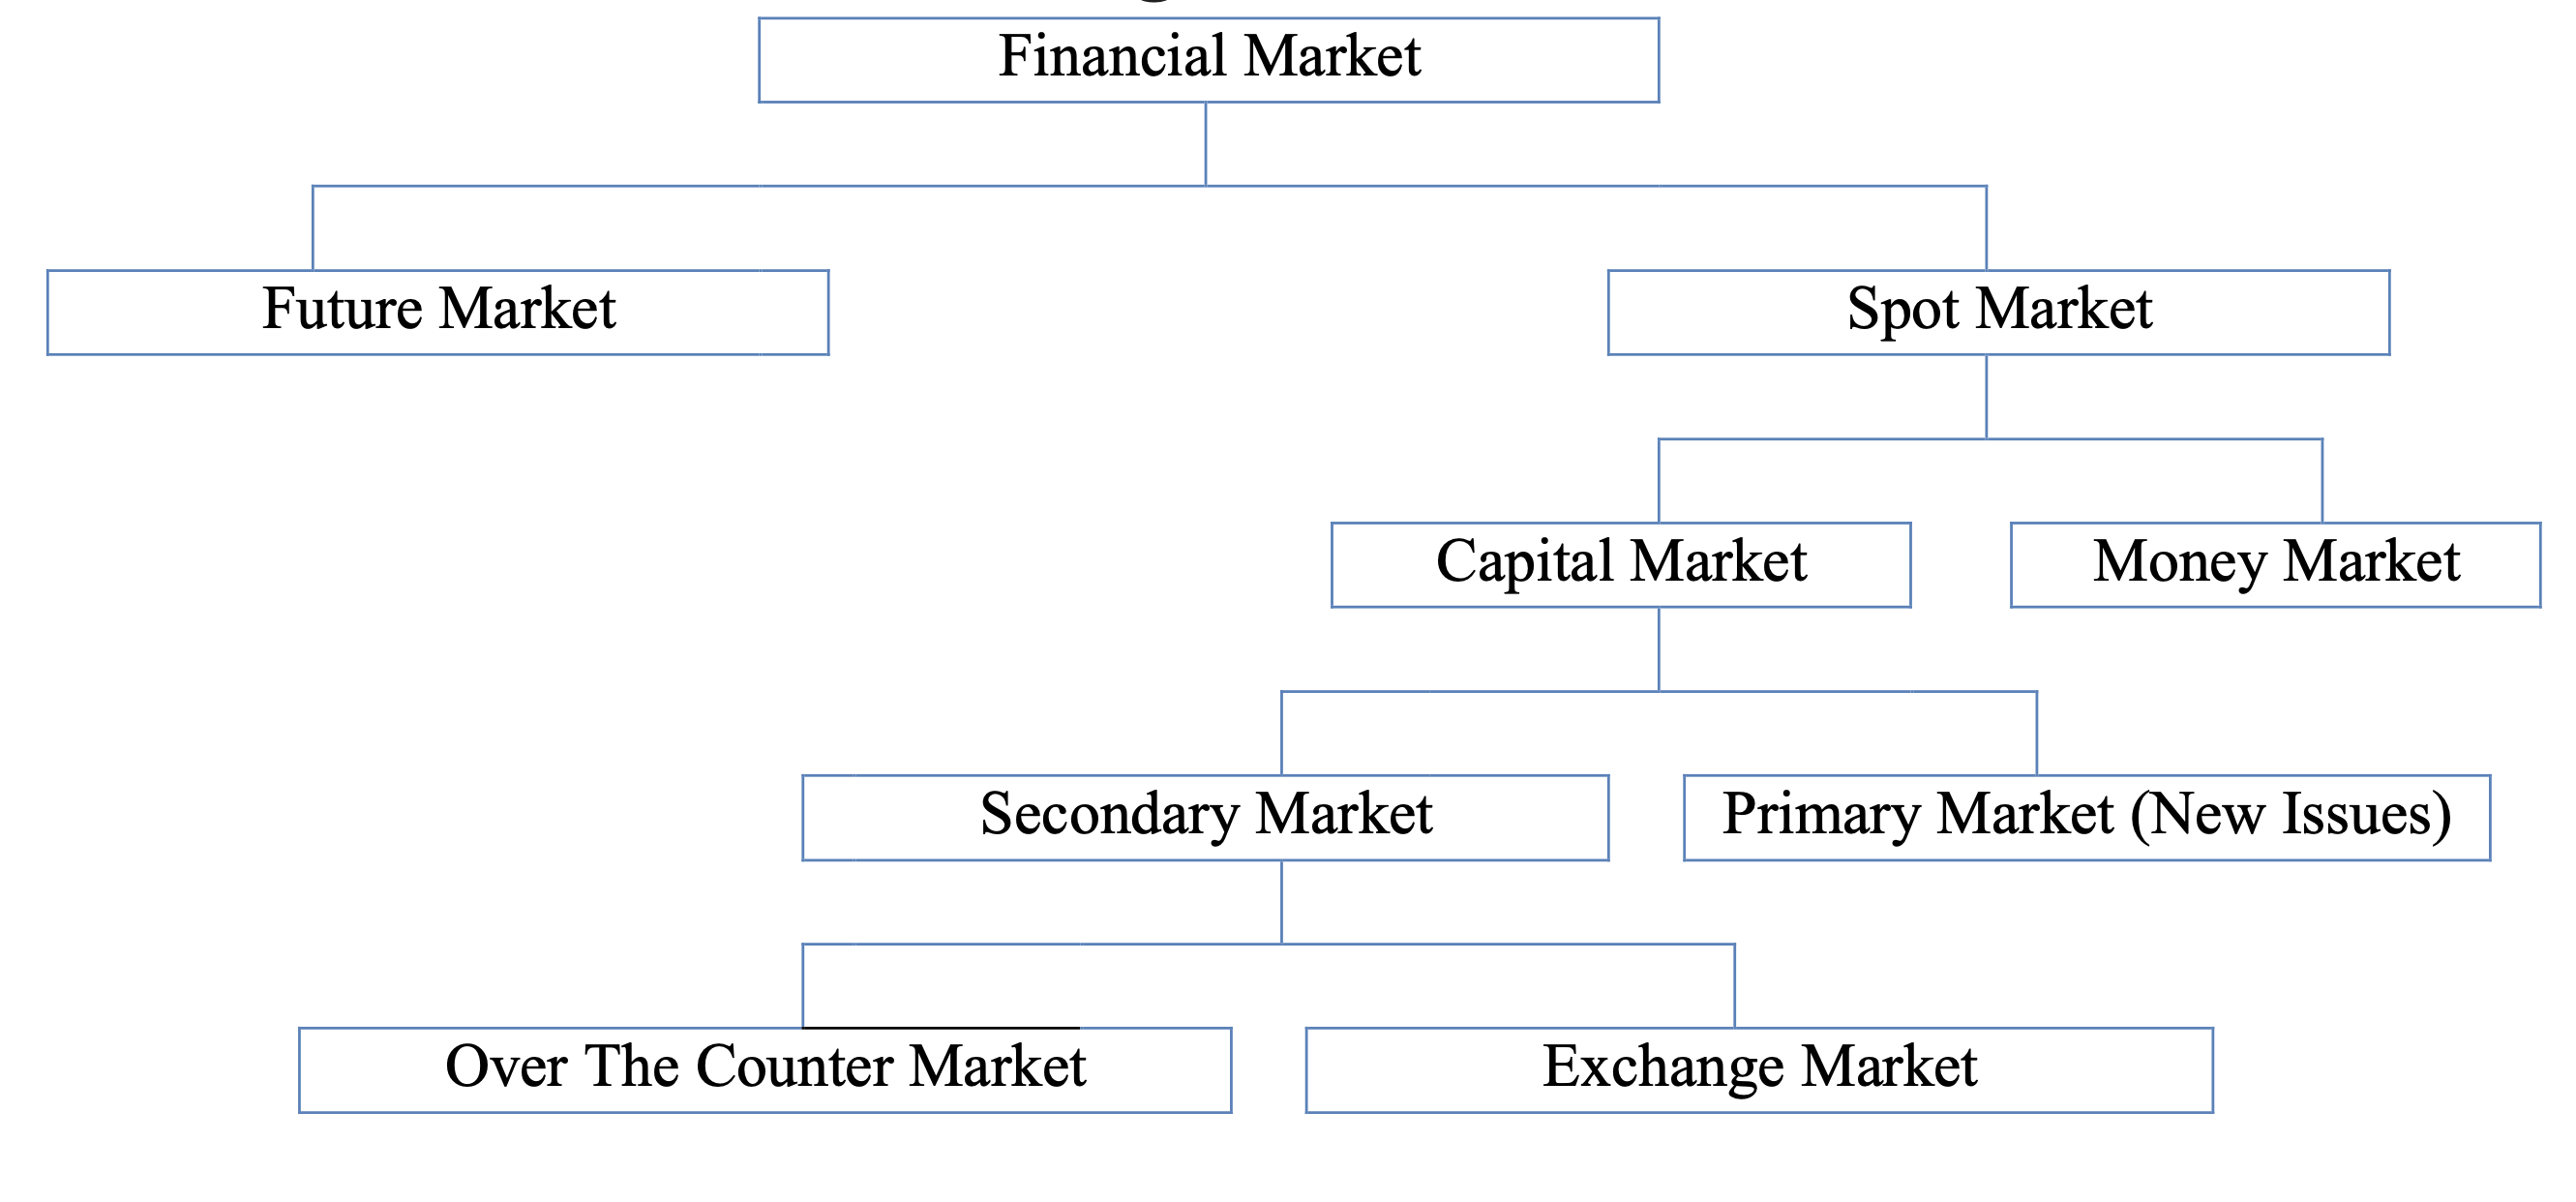
\includegraphics[width=\linewidth]{FIG2}
  \caption{Representation of financial markets}
  \label{fig:boat1}
\end{figure}

\subsection{Le marché au comptant et le marché à terme}
\begin{itemize}
\item Le marché au comptant est le marché sur lequel les matières premières ou les devises sont vendues au comptant et livrées immédiatement. On l'appelle aussi marché réel ou marché au comptant.
\item Le marché à terme, quant à lui, est la bourse où sont négociés les contrats à terme et les options sur les contrats à terme. Les bourses peuvent négocier des matières premières, des dérivés financiers ou une combinaison des deux. Des exemples d'échanges futurs incluent, Chicago Board of Trade (CBOT) et Chicago Mercantile Exchange (CME).
\end{itemize}

\section{Le marché au comptant}
Comme nous l'avons souligné ci-dessus, le marché au comptant est le marché sur lequel les marchandises sont vendues au comptant et livrées immédiatement. Il comprend à la fois le marché monétaire et le marché des capitaux.
\subsection{Le marché monétaire }
\begin{itemize}

\item Le marché monétaire est le segment du marché financier dans lequel sont négociés des actifs financiers à court terme (titres à moins d'un an d'échéance tels que les bons du Trésor, les certificats bancaires de dépôts, etc.). 
\item La plupart des transactions sur ce marché sont de grande taille, généralement d'un million de dollars (aux États-Unis) ou plus, et donc hors de portée des petits et moyens investisseurs. \item Les particuliers peuvent toutefois participer à ce marché par le biais de fonds communs de placement du marché monétaire. 
\item Les teneurs de marché tels que les grandes banques commerciales, les sociétés de courtage et les courtiers du marché monétaire facilitent la négociation de titres sur le marché monétaire. 
\item Les courtiers agissent principalement en tant qu'intermédiaires en rassemblant des acheteurs et des vendeurs potentiels et facturent une commission pour leurs services. 
\item Les courtiers, quant à eux, ont des positions actives sur les titres qu'ils traitent, en se tenant prêts à acheter (au cours acheteur) et à vendre (au cours vendeur) en fonction des besoins du client.
\item Certains des titres les plus importants du marché monétaire sont :
\begin{itemize}
\item Bons du Trésor
\item Certificats de Dépôts 
\item Papier commercial
\item Acceptations bancaires
\end{itemize}
\end{itemize}

\subsection{Le marché des capitaux}
\begin{itemize}
\item Le marché des capitaux est le segment du marché dans lequel les actifs financiers à long terme (titres à plus d'un an comme les obligations d'État et de sociétés, les actions, etc.) sont négociés. 
\item Les marchés des capitaux peuvent être subdivisés en deux : 
\begin{itemize}
\item le marché primaire 
\item le marché secondaire.
\end{itemize}
\end{itemize}
\subsubsection{Le marché primaire}
\begin{itemize}
\item Le marché primaire est la partie du marché sur laquelle s'effectue l'émission de nouveaux titres, souvent appelée marché des nouvelles émissions. 
\item Sur le marché primaire, les entreprises et autres organisations mobilisent les fonds dont elles ont besoin en émettant (vendant) des titres à long terme tels que des actions et des obligations à des investisseurs potentiels. 
\item Cependant, l'émission et la commercialisation de titres est une tâche spécialisée généralement entreprise par des institutions financières spéciales appelées banques d'investissement. 
\item Des exemples de certaines banques d'investissement bien connues sont Goldman Sachs, Merrill Lynch et Credit Suisse First Boston.
\end{itemize}
\subsubsection{Le marché secondaire}
\begin{itemize}
\item Le marché secondaire est le lieu où s'effectuent l'achat et la vente de titres déjà émis entre investisseurs. 
\item Ces opérations ne modifient pas le montant total des titres en circulation ; il transfère simplement la propriété d'un investisseur à un autre.
\end{itemize}

\section{Instruments de financement}
\subsection{Capitaux propres}
\begin{itemize}
\item La distinction clé dans les accords de financement est entre les capitaux propres et la dette. Le financement par capitaux propres représente les droits de propriété dans l'entreprise émettrice de capitaux propres et peut être levé soit au moyen d'une offre d'actions, soit en tant que bénéfices de l'année précédente investis en tant que bénéfices non distribués. 
\item Le financement par capitaux propres est essentiellement de nature permanente, car il est rare que les entreprises remboursent des capitaux propres.
\end{itemize}

\subsection{Emprunt}
\begin{itemize}
\item Le financement par emprunt représente un prêt de fonds à l'entreprise par un créancier. Un moyen utile de catégoriser la dette est en fonction de sa maturité. 
\item Par conséquent, la dette à très court terme est mieux représentée par un découvert bancaire ou un prêt à court terme,
\item Pour une dette à plus long terme, une entreprise peut contracter un emprunt bancaire ou lever des fonds en émettant une obligation. 
\item Les obligations peuvent être garanties sur les actifs de l'entreprise ou non garanties, ou elles peuvent être émises contre les flux de trésorerie entrants, ce qui est connu sous le nom de titrisation.
\end{itemize}


\begin{thebibliography}{1}

\bibitem{williams}
   Fabozzi, Frank J.
   \textit{Bond markets, analysis and strategies (9e édition)}.
 

% Uncomment the following lines to include a webpage
% \bibitem{webpage1}
%   LastName, FirstName. ``Webpage Title''.
%   WebsiteName, OrganizationName.
%   Online; accessed Month Date, Year.\\
%   \texttt{www.URLhere.com}

\end{thebibliography}

% --- Document ends here ---

\end{document}